\subsection{Moving window integration: maintained sum}
\label{sec:maintainedSum}

In the moving window integration filter, the filtered value $y_n$ is the average of the previous $N$ unfiltered values:
\begin{equation}
    y_n = \frac{1}{N} \left( x_{n- (N-1)}  + x_{n-(N-2)} + ... +  x_n \right) = \frac{1}{N} \sum_{k=-(N-1)}^{0} x_{n+k} = \frac{1}{N} S_n
\end{equation}

The following data point $y_{n+1}$ is based on the sum
\begin{equation}
    S_{n+1} = S_n + x_{n+1} - x_{n-(N-2)}
\end{equation}

If we maintain and update the sum $S$ as a variable, each new data point $y_{new}$ can be obtained by 
\begin{enumerate}
    \item Adding a new value $x_{\text{new}}$ to the sum $S$.
    \item Subtracting the oldest value $x_{\text{old}}$ from $S$.
    \item Dividing the sum by $N$, and returning the result.
\end{enumerate}

If $N=32 = 2^5$, we can bit shift $S$ by 5 instead of dividing by $N$. Bit shifting is cheaper than division computation-wise. In our C program for Assignment 1, we did not use the maintained sum approach, but we use the approach in our Gezel processor. To better compare the Gezel results with C results, we ran our C program with $N=32$, and included the results (Rpeaks, graphs) in this report. See section \ref{sec:conseq}.
\vspace{3cm}
\newpage
\subsection{Algorithm}
\label{sec:AlgIns}

%The algorithm for the filter can be seen as 3 steps. 
Our processor follows a 3-step algorithm to perform the moving window integration filter:

\begin{enumerate}
    \item The first step is loading and storing the data points $x_{\text{new}}$ and $x_{\text{old}}$. The external memory holds 250  data values, but we load them one-by-one to simulate a continuous flow of data. The new value is loaded from external memory into a register. Also to load the old data point into a register from the circular array located in RAM (illustrated on figure \ref{fig:circarray}). 
    
    \begin{figure}[H]
        \centering
        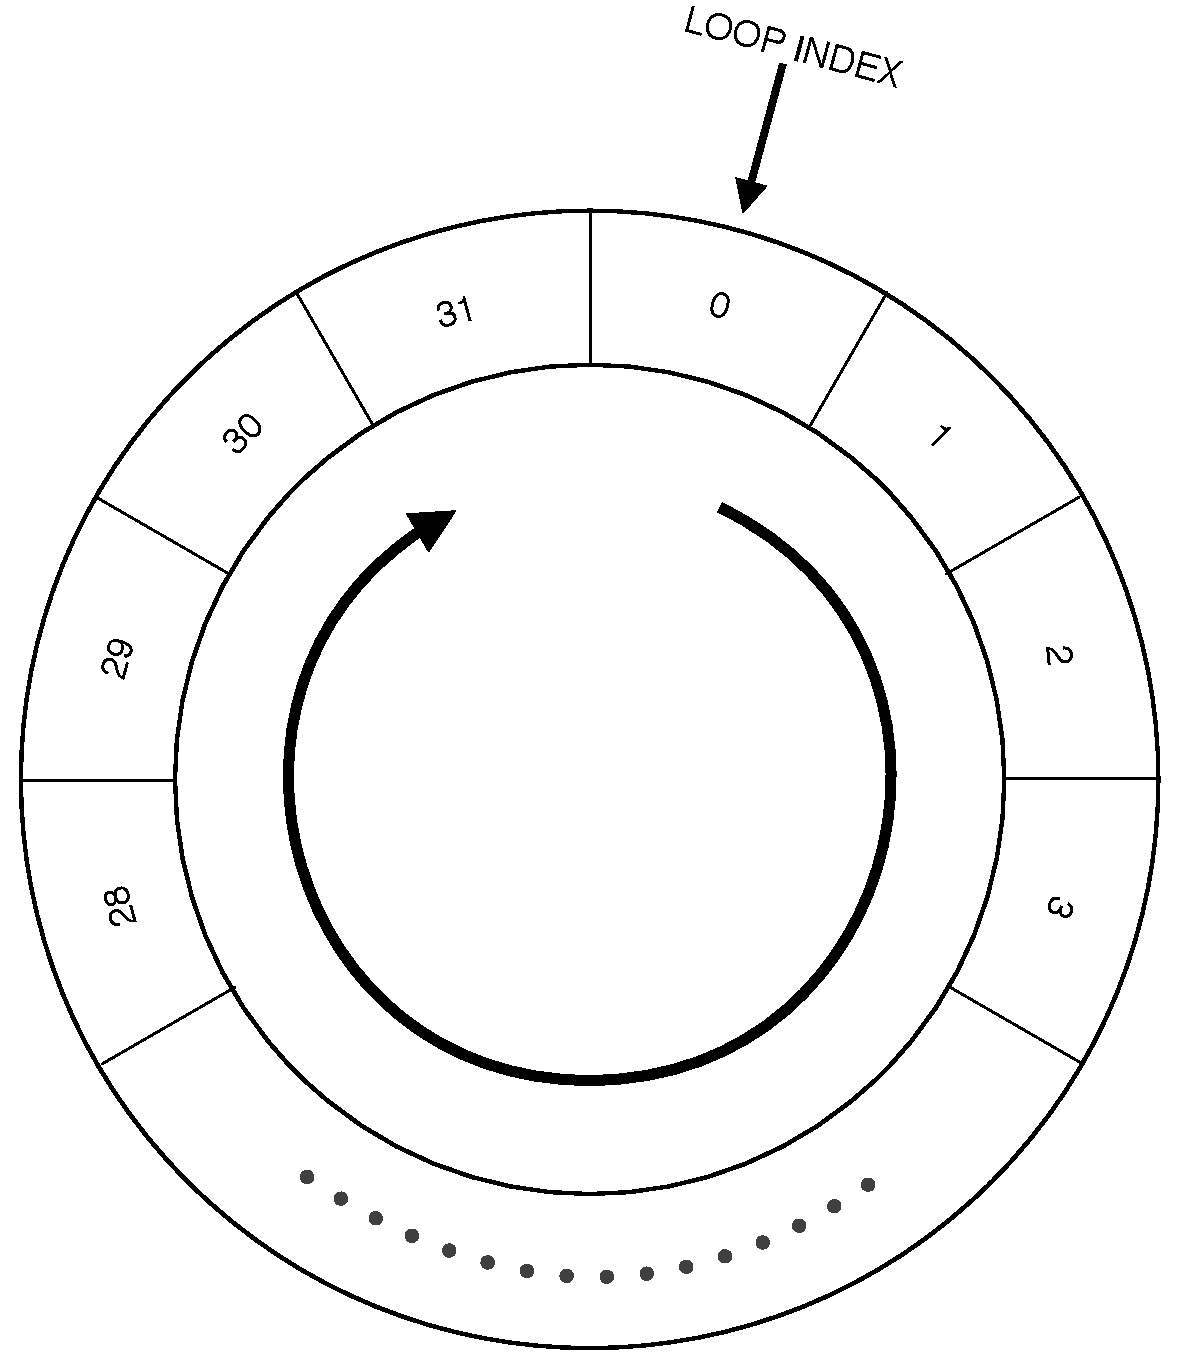
\includegraphics[width=0.5\textwidth]{1Design/fig/Circular_Array.pdf}
        \caption{Array to store the last 32 data points in memory. Whenever the index exceeds the last element, the index is reset, simulating a circular array.}
        \label{fig:circarray}
    \end{figure}
    
    %Before step two is explained, there are a few things we need to know. 
    The values in the circular array are initialized to 0 when the program starts. The sum $S$ of the elements in the circular array is kept in a register, and initialized to 0.
    %Since the sum of the array to begin with is zero by default, it is easily initialized. 
    
    \item The second step is computation. $x_{\text{new}}$ is added to the sum $S$, $x_{\text{old}}$ is subtracted, and the sum is bit shifted. The filtered data point (the bit shifted sum) is stored in separate register.
    % subtracting the old data point, adding the new data point to the sum, and bit shifting by 5 (equivalent to a division by 32). 
    
    \item The third and last step is preparing for the next round. Two counters are incremented: The address for loading data from external memory, and the index in the circular array. The latter may be reset, as explained in figure \ref{fig:circarray}. 
\end{enumerate}


When the program carries out the algorithm, the  instruction set in section \ref{sec:instructionSet} is used.

\subsection{Instruction set}
\label{sec:instructionSet}

\begin{table}[H]
    \begin{center}
    \begin{tabular}{|c||c|c|c|c|c|}
        \hline
        \textbf{Command} & \textbf{Opcode: ns(4)} & \textbf{AD1: ns(3)} & \textbf{AD2: ns(3)} & \textbf{AD3: ns(3)} & \textbf{Other: ns(3)} \\ \hline \hline
        \texttt{MOV}     & 0001          & Reg1       & ...        & Reg2       & ...          \\ \hline
        \texttt{ADD}     & 0010          & Reg1       & Reg2       & Reg3       & ...          \\ \hline
        \texttt{ADD1}    & 0011          & Reg1       & ...        & Reg1       & ...          \\ \hline
        \texttt{SUB}     & 0100          & Reg1       & Reg2       & Reg3       & ...          \\ \hline
        \texttt{BTS5}    & 0101          & Reg1       & ...        & Reg2       & ...          \\ \hline
        \texttt{INLP}    & 0110          & Reg1       & ...        & Reg1       & ...          \\ \hline
        \texttt{LOAD}    & 0111          & Reg1       & ...        & Reg2       & ...          \\ \hline
        \texttt{LOADC}   & 1111          & Reg1       & ...        & Reg2       & ...          \\ \hline
        \texttt{SAVEC}   & 1000          & Reg1       & Reg2       & ...        & ...          \\ \hline
        \texttt{SAVEX}   & 1001          & Reg1       & Reg2       & ...        & ...          \\ \hline
        \texttt{JMP}     & 1010          & ...        & ...        & ...        & ...          \\ \hline
    \end{tabular}
    \caption{Complete instruction set. Size is shown in the header. AD1: First chosen register. AD2: Second chosen register. Values from AD1 and AD2 are sent as two signals from \texttt{REG}. AD3: Which register to save incoming value to (from \texttt{ALU} or \texttt{SHUTTLE}, see figure \ref{fig:ComArch}).}
    \label{table:InstructionSet}
    \end{center}
\end{table}

The instructions have a bit size of 16. We chose this in order to represent it as a 4 digit hex number, since the \texttt{ipblock}\footnote{Preexisting library in Gezel, used to communicate with both internal and external memory.} reads in hex.

\subsection{Instruction definitions}
\label{sec:instructionDefinitions}

All references to registers follow table \ref{table:InstructionSet}.\\
\\
\textbf{Suffix:} The C in \texttt{LOADC} and \texttt{SAVEC} refer to \underline{c}ircular array. The X in SAVEX refers to e\underline{x}ternal memory.\\ 
\\
\textbf{Reg vs. R:} In the instruction set, the 3-letter notation Reg\_ (Reg1, Reg2 etc.) refers to the parameters required to follow the command. E.g. the \texttt{ADD} command requires 3 arguments (Reg1, Reg2, Reg3). When referring to a specific register in memory, the 1-letter notation R\_ (R0, R1 etc.) will be used.

\renewcommand{\arraystretch}{1.3}
\begin{table}[H]
    \begin{tabular}{rl}
    \texttt{MOV}:    & Store value from Reg1 in Reg2.                                    \\
    \texttt{ADD}:    & Add values from Reg1 and Reg2, and store the result in Reg3.        \\
    \texttt{ADD1}:   & Increment the value in Reg1 by 1.                                 \\ 
    \texttt{SUB}:    & Perform the subtraction Reg1 $-$ Reg2, and store the result in Reg3. \\

    \texttt{BTS5}:   & Bitshift value from Reg1 by 5 to the right, and store in Reg2.    \\
    \texttt{INLP}:   & Increment value in Reg1 by 1. Reset if value $\geq$ 31.\tablefootnote{Used for circular array index.}                \\
    \texttt{LOAD}:   &  Load value from memory at address Reg1, and store in Reg2.       \\
    \texttt{LOADC}:  & Load value from memory at address (Reg1 + 260), and store in Reg2.\tablefootnote{The circular array is stored at lines 260-291, skipping the original data list. This way the index can be kept at 0-31 but the address is shifted 260 places when loading from memory.}  \\
    \texttt{SAVEC}:  & At memory address (Reg1 + 260), store value from Reg2.\tablefootnote{The same way as the \texttt{LOADC} is shifted 260 places in memory, the \texttt{SAVEC} is shifted the same amount.}  \\
    \texttt{SAVEX}:  & At memory address (Reg1 + 300), store value from Reg2.\tablefootnote{The final result is placed 300 lines down, making sure not to overwrite important data. This way the \texttt{SAVEX} address can be the same as the \texttt{LOAD} address, only occupying one register.}      \\
    \texttt{JMP}:   & Jump. Change PC value to 4, resetting main loop.
    \end{tabular}
\end{table}
\renewcommand{\arraystretch}{1}

The instructions \texttt{MOV}, \texttt{ADD}, \texttt{ADD1}, \texttt{SUB} and \texttt{LOAD} are rather standard. But the others are customized to fit the exact purpose of the implemented algorithm.\\
\\
The instruction \texttt{BTS5} is used for bit shifting, but it can only bit shift 5 places to the right. This command is very important as it essentially divides a number by 32, used when computing the average $\frac{S_n}{N}$. The processor does not have a general instruction for division since only division by 32 is needed. \\
%, since it will divide by 32, going from the sum of elements to average value of all 32 elements. \\
\\
The shifting in \texttt{LOADC}, \texttt{SAVEC} (+260) and \texttt{SAVEX} (+300) is implemented to limit the resources spent on memory addresses.\\
\\
The \texttt{JMP} command is also heavily customized: It sets the PC value to 4. This corresponds to the first command of the loop (main loop, calculating data). Since the algorithm only needs one jump statement, it is hard coded to this value to keep the CPU as simple as possible.
